\chapter{The Standard Analysis Method for Resonance Finding}
\label{chapter:analysismethod}

\epigraph{\textit{But the truth can be re-found; most often it has already been written elsewhere.}}{--Jacques Lacan, Ecrits}
%TODO Adding Monte Carlo methods \\Edited
%TODO Gaussian process motivation
%TODO Fit function + swift method
%TODO Bayesian method for limit setting
%TODO Add fig:bump
% add to MC generation


\section{Introduction}
Both analyses presented in this thesis fall into the resonance search category, which are analyses that look for bumps like excesses on top of smooth backgrounds. The method is simple in its experimental signature, as can be seen in Figure~\ref{fig:bump} and theoretical calculation. Many particles have been discovered in this way before, which include the $J/\Psi$~\cite{PhysRevLett.33.1406}~\cite{PhysRevLett.33.1404}, the $\upsilon$~\cite{Herb:1977ek}, the $W$~\cite{Arnison:142059}, $Z$~\cite{hollik1984composite}, and the Higgs boson. The method has great potential in making future discoveries. This chapter describes
the analysis methods used in performing the analyses covered in Chapter~\ref{chapter:dijetISR} and Chapter~\ref{chapter:dimuon}. 

These analyses perform searches in the resonance mass variable. The variable came from the addition of the 4-vector of the two candidate final state particles.

\begin{figure}[!htb]
    \begin{center}
        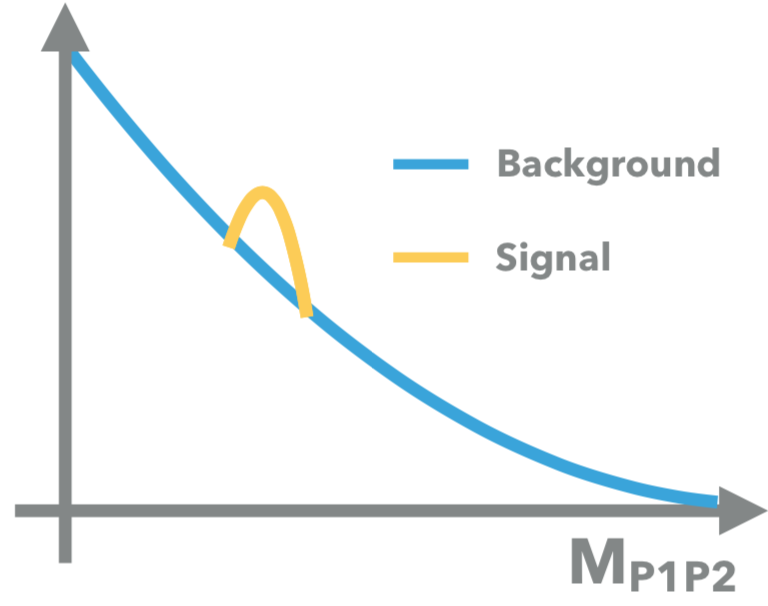
\includegraphics[width=0.75\textwidth]{figures/chapter_analysismethod/resonance}
        \caption{
            This cartoon illustrates a typical resonance finding experimental signature in the resonance mass variable. 
        }
        \label{fig:bump}
    \end{center}
\end{figure}
\FloatBarrier

The chapter below provides a recipe for a resonance finding analysis: Monte Carlo generation(MC) is used to aid statistical procedure formulation. Its generations are detailed in Section~\ref{sec:MC}. Proper data preparation required for both the data and the MC before statistical analysis is discussed in Section~\ref{sec:dataprep}. The background estimation method and their verification tests are given in Section~\ref{sec:backgroundest}. The search for resonances as excesses is quantified statistically. Two separate statistical statements, one on excess finding, and the other one on signal strength upper limit setting are discussed in Section~\ref{section:stats}. 

\section{Simulated Physics Events(Monte Carlo)}
\label{sec:MC}
Simulated physics events(Monte Carlo) are used to design the cuts which optimize the selection, verifying the validity of the data-driven background estimation strategies as well as deriving the different systematic uncertainties(E.G. luminosity uncertainty) present in the experiment.
An event generator used by ATLAS is PYTHIA~\cite{PYTHIA}, which is used to simulate the proton-proton collision, the tree-level generation, the hadronization, the fragmentation as well as the showering. 
Other than PYTHIA, the PowHeg generator~\cite{oleari2010powheg} and NLOJet++~\cite{nagynlojet++} are also used. The detector effect is simulated by GEANT4~\cite{Agostinelli:602040}.

%It uses different \textit{tunes}, which are models and their parameters to estimate the effect of pile-up and the effect of simulated ``next-to-leading-order" showering. 


\section{Data Preparation}
\label{sec:dataprep}
The data of the analyses discussed in this chapter originate from collision data. It is collected from the ATLAS detector and its triggering hardware and software discussed in Chapter~\ref{chapter:ATLAS}. The data collected as energy deposits and tracks are analyzed and collected analysis objects as discussed in Chapter~\ref{chapter:common_analysis_items}. After that, the dataset goes through several more steps in data preparation before getting analyzed for resonance finding in the chapter: the following is a short outline of how data are being prepared for the analyses.

First trigger chains addition is studied, balancing both events collected and signal sensitivity of the dataset studied. After that, the data is processed with the optimal analysis object working points applied, then, event cuts are introduced to maximize the signal sensitivity while reducing the background events. The resolution of the data collected from detector is constrained by detector resolution, a binned approach is taken. The binning is selected based on studies on the detector resolution and signal sensitivity consideration. Details is described in Section~\ref{sec:binning}). Finally, a cross-check that compares the data and MC is performed variable regions other than the targetted spectrum. An agreement between MC and data ensures both the previous steps in data preparation are executed correctly and the MC modelling is close enough to data descriptions. After all the data preparation steps are completed, a target signal spectrum is available to be analyzed statistically for resonances. 

\subsection{Binning Strategy} 
\label{sec:binning}

The target spectrum is binned for the resonance hunt. The bins are chosen to be narrower than the width of the expected signal, as this would lower the probability of mistaking fluctuation in a single bin as excess.

The binning is optimized through the mass resolution of the target spectrum. Since mass resolution describe the maximal sensitivity seen in the target spectrum, binnning is often chosen to be factors of the maximal resolution. This avoid the lost of information and allow the signal bump to be wider. 
The mass resolution is found through MC studies. As its main contributor is the detector response, it can be studied through by performing a Gaussian fit on the $m^{reco}-m^{truth}$ on MC sample, where $reco$ is reconstructed event from GEANT4, and $truth$ is the truth events showering and detector reconstruction from the same event.
A Gaussian fit is performed to find the mean ($\mu$) and the width($\sigma$). The width found for the particular reconstructed mass is the resolution at that mass. 

%A uniform binning is chosen for the dimuon analysis, as it would make the background estimation more simplified. For the dijetISR analysis, to cope with the low statistics in the high mass region, variable bin size based on detector resolution is used. 

\section{Background Modeling}
\label{sec:backgroundest}
After the dataset has been prepared, the spectrum is ready to be analyzed to search for resonances. In order to analyze statistically whether there is an excess of events beyond the Standard Model prediction, a reliable prediction of the Standard Model events in the signal region along with its statistical error is needed. The step to estimate background Standard Model events is known as background modeling.
Many considerations go into background modeling for analysis: accuracy, availability, size of the estimation error and ease of implementation. In ATLAS, the following methods are recommended for background modeling in order of descending preference:
    First, the background estimation can be found by the MC generation of the events when the simulation is reliable and inexpensive for data generation. Second, in cases where the MC generated is low in event count but reliable in shape, an alternative estimation could be executed by scaling up the template from MC. In the case of the two analyses presented in this thesis, neither are there enough MC events nor are the shape of the MC event physically reliable. Thus, another class of methods of background estimation needs to be explored, all relying on the ``smoothness" feature of the background events. These include the fit function method, the expanded sliding window fit method(SWiFT) and the Gaussian Process method~\cite{frate2017modeling}.
    In the following section, the fit function method, the SWiFT method and the Gaussian Process method are discussed.

\subsection{Fit Functions/Global Fit}
\label{sec:fitfunction}
A class of fit functions are used to describe the distribution of the reconstructed mass due to smooth background. The most commonly used forms are cited as the following~\cite{ATL-PHYS-PUB-2020-028}. The selected fit functions are all resistant to capturing localized excess.

    \begin{itemize}

    \item \textbf{Polynomial}
        \begin{equation}
            f(m)= a_0 + a_{1}m + a_{2}m^{2}+...
        \end{equation} Here, m is the resonance mass, and $a_{i}$ are the different parameters.
    \item \textbf{Power Laws}
        \begin{equation}
            f(m)= a_{0}m^{b}
        \end{equation}

    \item \textbf{Exponentials}
        \begin{equation}
            f(m) = a_{0}e^{-b_{0}m} +a_{1}e^{-b_{1}m}+...
        \end{equation}
    \end{itemize}

From the above foundation, a list of historic fit functions has been developed over the years~\cite{Pachal:2063032}.
    %TODO cite 

    \begin{equation}
        f(m)=\frac{p_{0}}{m^{p_{1}}}e^{-(p_{2}m+p_{3}m^{2})}
    \end{equation}See~\cite{UA2:1990gao} for details.

    \begin{equation}
        f(m)=\frac{p_{0}}{m^{p_{1}}}(1-\frac{m}{\sqrt{s}})p_{2}
    \end{equation}See~\cite{1995} for details.

    \begin{equation}
        f(m)=\frac{p_{0}}{m^{p_{1}}}(1-\frac{m}{\sqrt{s}}+)p_{2}
    \end{equation}See~\cite{b582dc2d9c234174bfe2adbc9729bf42} for details.

    \begin{equation}
        f(m)=p_{0}(1-x)^p_{1}x^{p_{2}+p_{3}ln(x)}
    \end{equation}See~\cite{2009} for details.

    \begin{equation}
        f(m)=(1-x)^{p_{0}}x^{p1+p2ln(x)}
    \end{equation}See~\cite{2014} for details.

    In these fit functions, m is the resonance mass, p are the parameters, and x is defined to be $\frac{m}{\sqrt{s}}$.

\subsubsection{Cross-validation}
K-fold cross validation is often used to ensure the fit function is chosen correctly. In the procedure, the original dataset is divided into k different equal event size subsets through a random draw from the original dataset. Each of these subsets is tested by the candidate fit function and validated on the validation set. The best fit is chosen by averaging the $p$-value of the fit test statististic, $\chi^{2}/NDF$. The best fit is defined to have a $p$-value of the closest to 0.5.

While the fit function is relatively easy to implement, it is highly restrictive for complicated background shapes since it is low in flexibility~\cite{ATL-PHYS-PUB-2020-028}. Making the background modelling on data inaccurate. When the increased luminosity of the LHC dataset leads to difficulties in fitting the background accurately, SWiFT and Gaussian Process are developed for the challenge. 

    \subsection{Sliding window fit(SWiFT)}
    When the simple fit function failed to model the data, SWiFT can increase the fit flexibility and the degree of freedom by fitting multiple narrower windows rather than the entire spectrum. The SWiFT window fitting procedure is summarized as below:
    
    1. A global fit is performed in the overall spectrum. Only when the overall $\chi^{2}$ $p$-value is below 0.01, SWiFT is attempted. Otherwise, the procedure ends in this step and a global fit method will be used. 

    2. The SWiFT fit will start with the maximum sized window, which is the number of bins of the entire spectrum minus one. The window scan starts from the lowest mass region along the spectrum. A fit is performed in the window. This estimates the spectrum up to the middle point of the window.

    3. The window moves up by one bin along the resonance mass spectrum. Another fit is performed. The prediction up to the middle of the window is piece-wise appended to the prediction in step 2. 

    4. Step 3 is repeated, until the end of the spectrum is reached. The final fit is checked against the threshold $p$-value of the $\chi^{2}$. If the fit $\chi^{2}$ is below the designated threshold, the background estimation ends. Otherwise, the window size is further reduced by one bin, and step 2 and 3 are repeated until either a fit with a bumphunter $p$-value 0.01 is found or the minimum window size is reached. The minimum window size is defined by the signal injection test discussed
    below in Section~\ref{sec:signalInjection}.

    Figure~\ref{fig:swift} here shows a doodle of the sliding window method.
    While the SWiFT can provide extra flexibility to the fit for better accuracy, it is also prone to becoming too flexible. Signal present in the data could be estimated as part of the background model. This would lead to diminished signal sensitivity. To provide the most accurate background prediction while balancing signal sensitivity, SWiFT always aims to use the largest window possible that can still accurately describe the background and a study is done (the signal injection test) is performed to find the smallest window that can be used that still provide enough signal sensitivity for the search.

The SWiFT window size is not selected until the data is unblinded, to aid the use of the largest possible window size. A carefully designed unblinding procedure is required to select the optimal window size for the estimation. Figure~\ref{fig:unblinding} shows a sample unblinding procedure, as used in the dijetISR resolved analysis in presented in Chapter~\ref{chapter:dijetISR}.

\begin{figure}[!htb]
    \begin{center}
        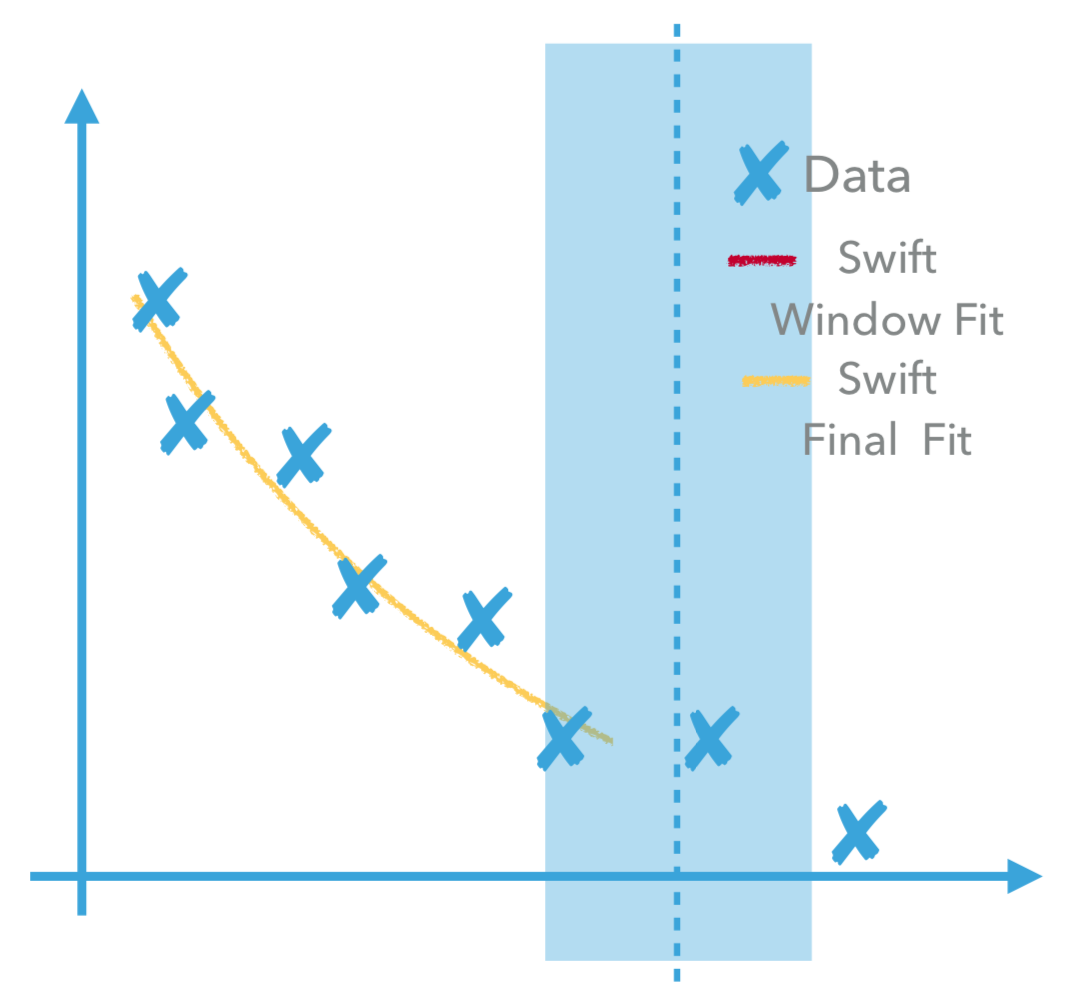
\includegraphics[width=0.75\textwidth]{figures/chapter_analysismethod/swift2}
        \caption{
            This figure shows a doodle on the procedure of the sliding window fit. 
        }
        \label{fig:swift}
    \end{center}
\end{figure}

\begin{figure}[!htb] \begin{center}
        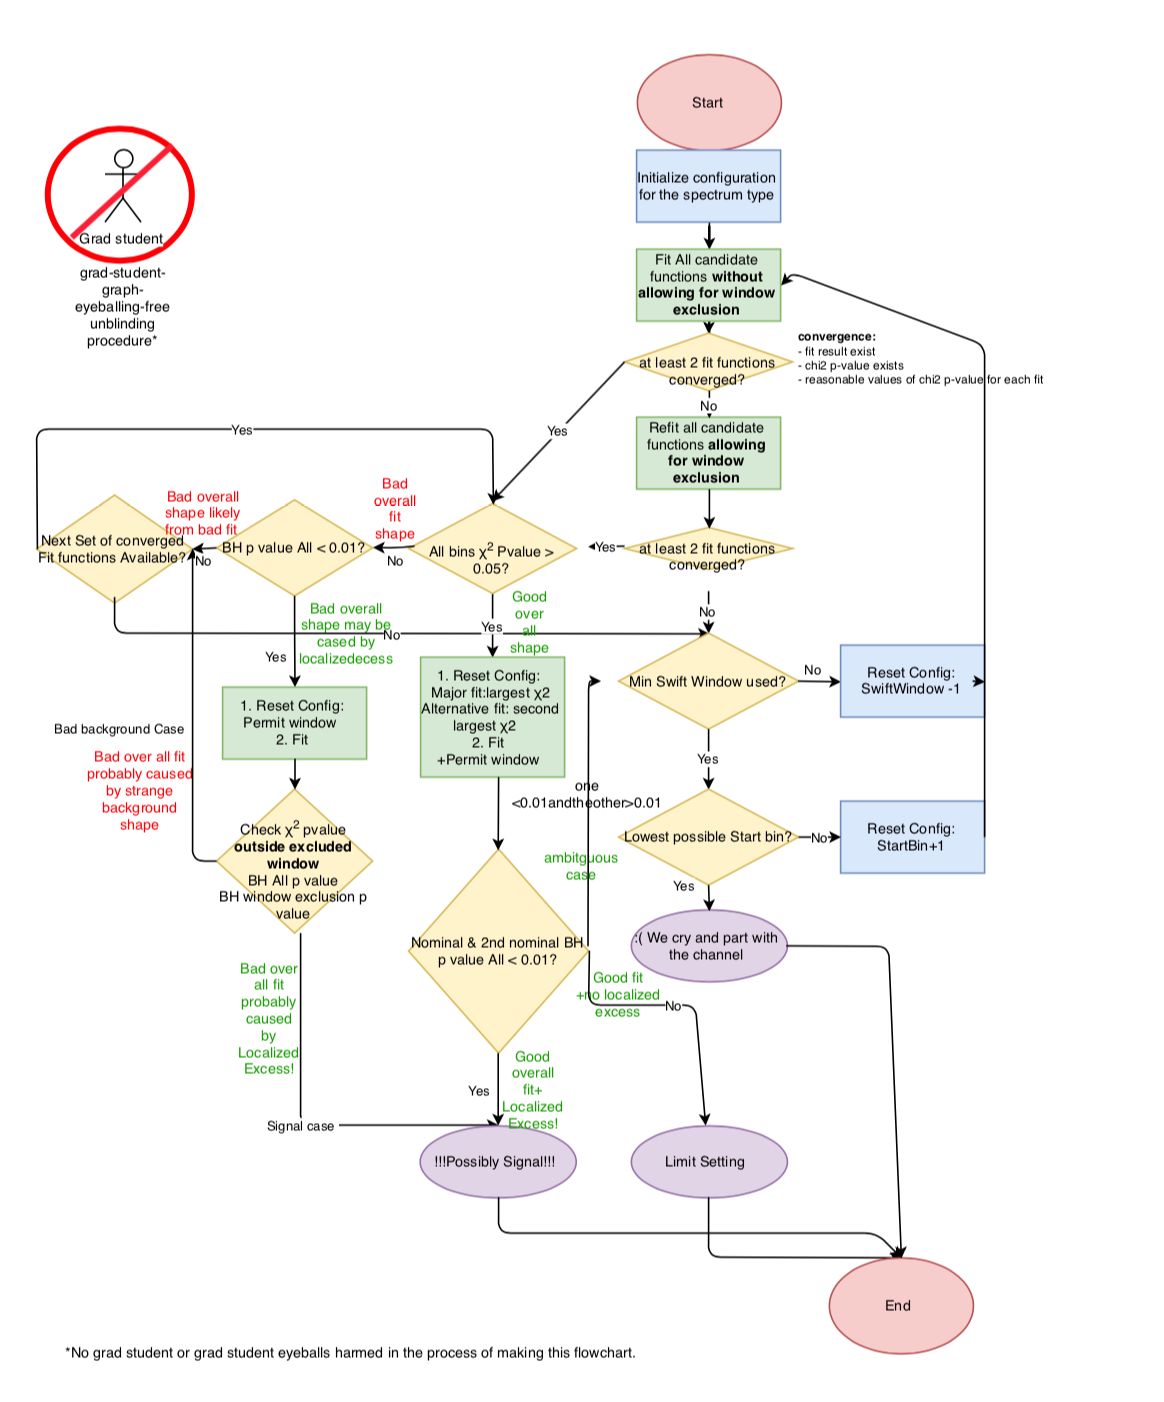
\includegraphics[width=1.05\textwidth]{figures/chapter_analysismethod/swift_unblindingflowchart}
        \caption{
            This figure shows a doodle on the procedure on the unblinding using SWiFT.
        }
        \label{fig:unblinding}
    \end{center}
\end{figure}
\FloatBarrier
    
    \subsection{Gaussian Process} 
    \label{sec:GP}

    Gaussian process background prediction is performed through Bayesian inference. The prior Gaussian joint probability distribution form more constricted posterior distribution with the added information from data. Unlike the above fit function-based method, Gaussian Process predicts an infinite number of functional forms, constrained by a kernel, which defines the bin-to-bin covariance.



    Gaussian process can naturally be applied to the background estimation of a spectrum since the bin event count in background and signal modeling are approximatedly a Gaussian distribution in each bin: In the resonance spectrum background, the prediction in every bin is a Poisson distribution due to its counting experiment nature. Poissonian distributions can be approximately described as a Gaussian Distribution through the Central Limit Theorem~\cite{kwak2017central}. As the distribution between the points is smooth, the relationship between each of the neighboring bins can be described by a joint distribution where the correlation is a covariance matrix. The Gaussian process allows for more flexibility in the functions compared to the above two methods, as can be shown here in this covariance matrix diagram:

    \begin{figure}[!htb]
        \begin{center}
            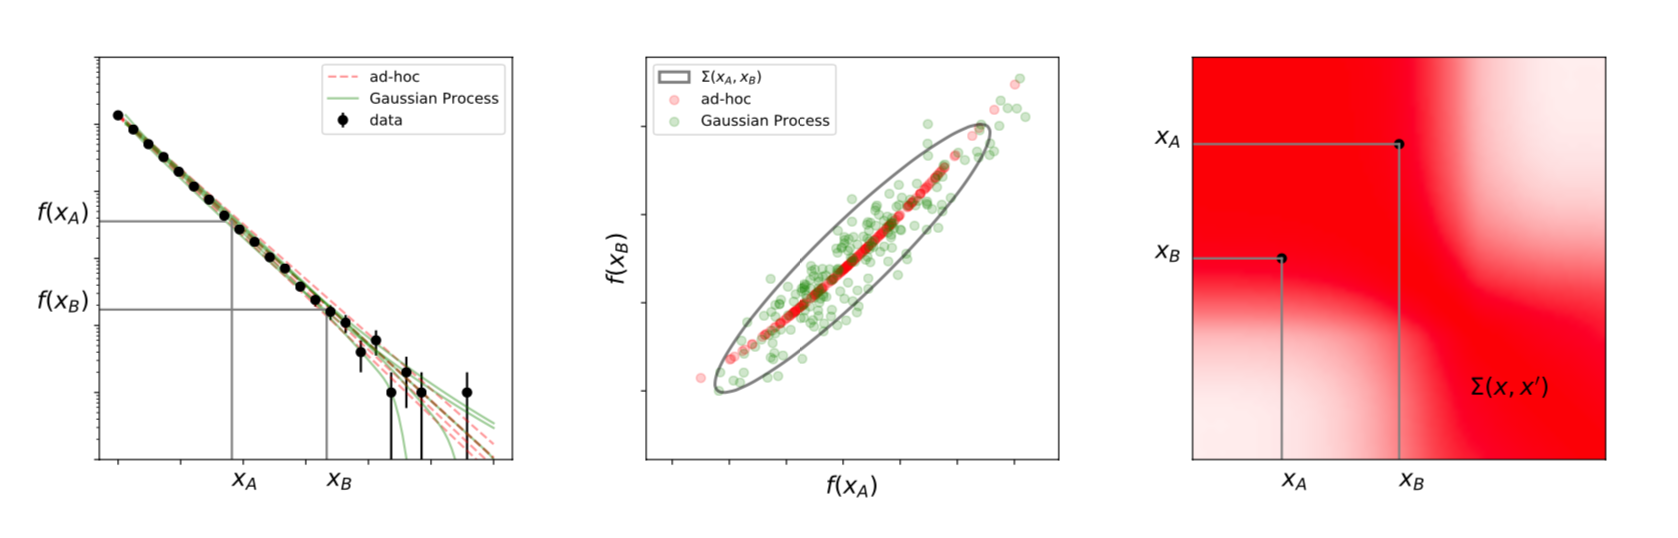
\includegraphics[width=0.7\textwidth]{figures/chapter_analysismethod/GP}
            \caption{
                These figure shows that the Gaussian process fit is able to provide more flexibility than the standard fit function method. The Red line in the first panel shows results from the fit function method and the green line shows the extra flexibility gained by Gaussian Process. The second pane shows that the possible value of the fit functions are relatively constricted (in red) compared to the Gaussian Process prediction (green) when the prediction are sampled at point $X_{A}$ and $X_{B}$. The black line shows the covariance matrix. The third pane shows the Covariant matrix of the kernel, where $X_{A}$ and $X_{B}$ are labeled. ~\cite{frate2017modeling}.
            }
            \label{fig:GaussianProcess}
        \end{center}
    \end{figure}
    \FloatBarrier


\subsubsection{Gaussian Process: Regression}

The Gaussian process background prediction method is a Bayesian method that predicts the posterior probability distribution. The mean function of this posterior probability distribution is the backgrdoun estimation prediction from GP, and the covariance matrix from it is the GP prediction error.

%where the prior distributions can be ``updated" by binning information. From Bayesian inference, a new prediction can be formed from the posterior. It can be shown that the mean and covariance can be given by the following formulae:

    \begin{itemize}

        \item \textbf{The Mean Function}

    \begin{equation}
        \mu(x_{*}|y)  = \mu(x_{*})+ K(x_{*}, x)[K(x, x)+ \sigma^{2}(x)I]^{-1}(y-\mu(x))
    \end{equation}
    Here, $\mu(x_{*}| y) $ is the mean function posterior prediction of of point $x_{*}$, given known data point x and y, K is the kernel, $I$ is the diagonal matrix, $\sigma$ is the white noise term in each bin. $\mu(x_{*})$ is the prior probability distribution mean. $x$ is a vector of the input mass point, and $x'$ are the same points in a 2d matrix.

    \item \textbf{The Covariance Function}
    \begin{equation}
        \sum(x_{*}, x_{*}') = K(x_{*}, x) - ((K(x_{*}, x')+\sigma^{2}I)^{-1)}[K(x, x')]
    \label{eq:covariance}
    \end{equation}  
    Here, the covariance is defined for $x_{*}$ and $x_{*}'$, the data point where the predictions were made, x and x' where the input data points are given. K is the kernel of the Gaussian Process prediction.

    \end{itemize}

    Here, x and y are input data to constrict the distribution, $x_{*}$ is the points where the posterior GP are evaluated from, x' is the same points as x in a 2d matrix.

    \subsubsection{Gaussian Process: the Kernel}
\label{sec:kernel}
From Eq.~\ref{eq:covariance}, kernel is directly related to the covariance function in Gaussian Process. Kernel descibes how the relating neighboring points are related to one another. 
Various kernels are used for different analysis backgrounds with distinct features. A specific example to the dijet spectrum is demonstrated in ~\cite{frate2017modeling}.

%t's found that the simple radial basis function and a white noise kernel are sufficient to describe the background spectrum, the signal is described by another radial basis function kernel of a particular mean value.
%The kernels are given as the following: 
An other more general example is given as below.
%
    \begin{itemize}
        \item \textbf{Background Kernel}

            The background kernel is the addition of the Radial Basis kernel function plus the white noise kernel.
            \begin{equation}
                K_{bkg}(x, x') = A_{1} * exp(-\frac{||x-x'||}{2\sigma^{2}}) *+ K_{noise}
                \label{eq:backgroundkernel}
            \end{equation}
            Here, $A_{1}$ is the amplitude hyperparameter that describes the size of the kernel, $\sigma_{1}$ is the lengthscale parameter.
            The noise kernel is a constant diagonal kernel:
            

			\begin{equation}
            K_{noise}(x_{i}, x_{j}) =
			\begin{cases} \text{noise level} & \text{if $x_{i}==x_{j}$,} \\
			\\
            0 & \text{otherwise.}
			\end{cases}
			\end{equation}

        \item \textbf{Signal Kernel}

            The signal kernel is a square centered exponetial kernel
            \begin{equation}
            K(x_{i}, x_{j})=A_{2}\cdot exp(-(x-m)^{2}/(2\cdot\sigma_{2}^{2}))\cdot exp(-((x'-m)^{2}/(2\cdot\sigma_{2}^{2}))) + K_{noise}
            \label{eq:signalkernel}
            \end{equation}

    \end{itemize}
            Here, $A_{2}$ is the amplitude of the signal kernel, m is the value where the kernel peaked on, and $\sigma_{2}$ is the lengthscale of the signal kernel. 

	Of all the hyperparameters, lengthscale($\sigma$) is given special attention as its value descirbes how much neighboring points affect prediction at any given point. Its special treatment is described in the following sections.

    \subsubsection{Gaussian Process: Hyperparameter Optimization}
    \label{sec:hyperparam}
    %The lengthscale($\sigma$) hyperparameter in both kernels(See Eq.~\ref{eq:backgroundkernel} and Eq.~\ref{eq:signalkernel}) is prone to overfitting when the chosen value is too small. This would lead to reduced signal sensitivity and the overfitting of statistical fluctuation. A lower bound is set in these hyperparameters: The lower bound in the background kernel lengthscale is determined by the signal injection test described in Section~\ref{}; the lower bound in the signal kernel lengthscale
    %is chosen through the binning studies in Section~\ref{sec:binning} respectively. 
    Kernels are parametetrized by hyperparameters. Hyperparameters are higher level parameters that controls and aid the learning of the process through input of data. The lengthscale hyperparameter, with its special nature, has a lower bound, found through the signal injection test described in Section~\ref{sec:signalinjection}. Other hyperparameters are not bounded. The minimization of the hyperparameters is performed through a scalar conjugate gradient search. To avoid reaching a local minimum, the initial values of the hyperparameters are chosen through a grid before the minimization. The minimized hyperparameter are compared to the other sets. The set of value with the overall lowest negative log likelihood is chosen to be the optimal hyperparameters.
%In fitting of a mass spectrum and its signal. The kernel hyperparameters are allowed to float and the final values are optimized through the scaled conjugate gradient algorithm, which minimizes the negative log marginal likelihood of the Gaussian Process:

    \begin{equation}
        -\ln(L) = -\frac{1}{2} ln |\sum| - (y-\mu(x) ) - \frac{n}{2}\ln(2\pi)
    \label{eq:loglikelihood}
    \end{equation}
    

    In this Gaussian process testing procedure, the hyperparameters are first found on a test fit on the variation of MC, the fixed hyperparameters are then applied to data.
%
%\subsection{Background Fitting Tests}
%Following the ATLAS smooth background recommendation~\cite{ATL-PHYS-PUB-2020-028}, the following tests are performed to ensure the validity of the background estimation for resonance searches.

%\subsubsection{Signal Injection Test}
%\label{sec:signalInjection}
%
%    Increasing the number of parameters in a fit function, using smaller windows size in SWiFT, or using a background kernel lengthscale in the Gaussian Process all increases flexibility in modeling the background. However, the increased flexibility in background modeling often comes with the price of decreased signal sensitivity. An overly flexible background estimation would fit the signal away as part of the background. 
%    Therefore a test to quantifies the signal sensitivity of the background estimation is necessary. The test is called the signal injection test. On ATLAS, it is required that the background modeling provides sensitivity to signals of at least 3 $\sigma$ of the background error.
%
%    The background error is defined by the generation of 10,000 bin-by-bin Poissonian toys from the original background MC spectrum, and by refitting the toys by Gaussian Process background kernel estimation. A Gaussian fit is performed on the prediction of each bin, the resulting width of the Gaussian fit in each bin is defined to be the 1 $\sigma$ background estimation. 
%
%    %defined by the width of the Gaussian envelope from the pseudoexperiment fits. The background estimation passes the signal injection test when it passes such requirement.
%
%    In addition to quantifying signal sensitivity, the signal injection test is used to constrain the lower bound of the lengthscale in Gaussian Process and SWiFT window size. The window size or lengthscale value is restricted by to a lower bound that would return a background estimation that provides sensitivity to signals of at least 3 $\sigma$ background error in size.
%
%    Signals of different mass widths are generated from a Gaussian distribution. Poissonian noise is thrown randomly on the distribution to create a pseudo signal distribution. The mass widths are chosen to be 1\%, 3\% and 5\% respectively. Signal of different scales with corresponding error is generated and is injected into the background MC distribution.
%
%    For each chosen maximum lengthscale/SWiFT window, and different signal widths, the below is performed with the bumphunter.
%
%   1. First a background fit is performed on the background MC distribution, the bump-hunting~\cite{choudalakis2011hypothesis} procedure is performed as described in the above section. If the overall bumphunter $p$-value are below the critical value for window exclusion, the next step is performed. Otherwise, the background fit strategy has to be reviewed. A different fit function or Gaussian Process kernel is needed.
%
%   2. A small signal is injected in the background MC distribution, a fit is reperformed, and the bumphunter window and overall $p$-value is calculated again. 
%
%   3. An increasing signal size is injected into the spectrum and step2 is repeated until a signal of size large enough to lead to a small enough bumphunter statistic $p$-value.(The test statistic is defined in Section~\ref{teststatistics}) When the $p$-value is below 0.01, window exclusion in the bumphunting procedure is triggered. The signal size injected just before the window exclusion is the largest signal the search is not sensitive to. The minimal signal size injected that triggers the window exclusion is the smallest signal size that the search is sensitive to. 
%
%
%%Starting with the smallest signal size and the smallest width, the bumphunter procedure detailed in section~\ref{} is ran on the signal injected background MC. The signal size injected increases, until the bumphunting procedure finds a window with bumphunter statistic $p$-value $<$ 0.01 that a bumphunter window exclusion is triggered. The size of the signal injected right before the window exclusion triggering is the ``just below"
%%triggering signal size, and the signal size that triggers the window exclusion is known as the ``just above" signal size. The "just below"
%%window size is the largerst signal that the background estimation is not sensitive to; and the ``just above" signal size is the smallest signal that the background estimation is sensitive to. When the background kernel lengthscale is chosen to be 4 GeV, the background model is sensitive to signal 3 $\sigma$ or above in background error. 
%%
%
%%\begin{figure}[!htb]
%%    \begin{center}
%%        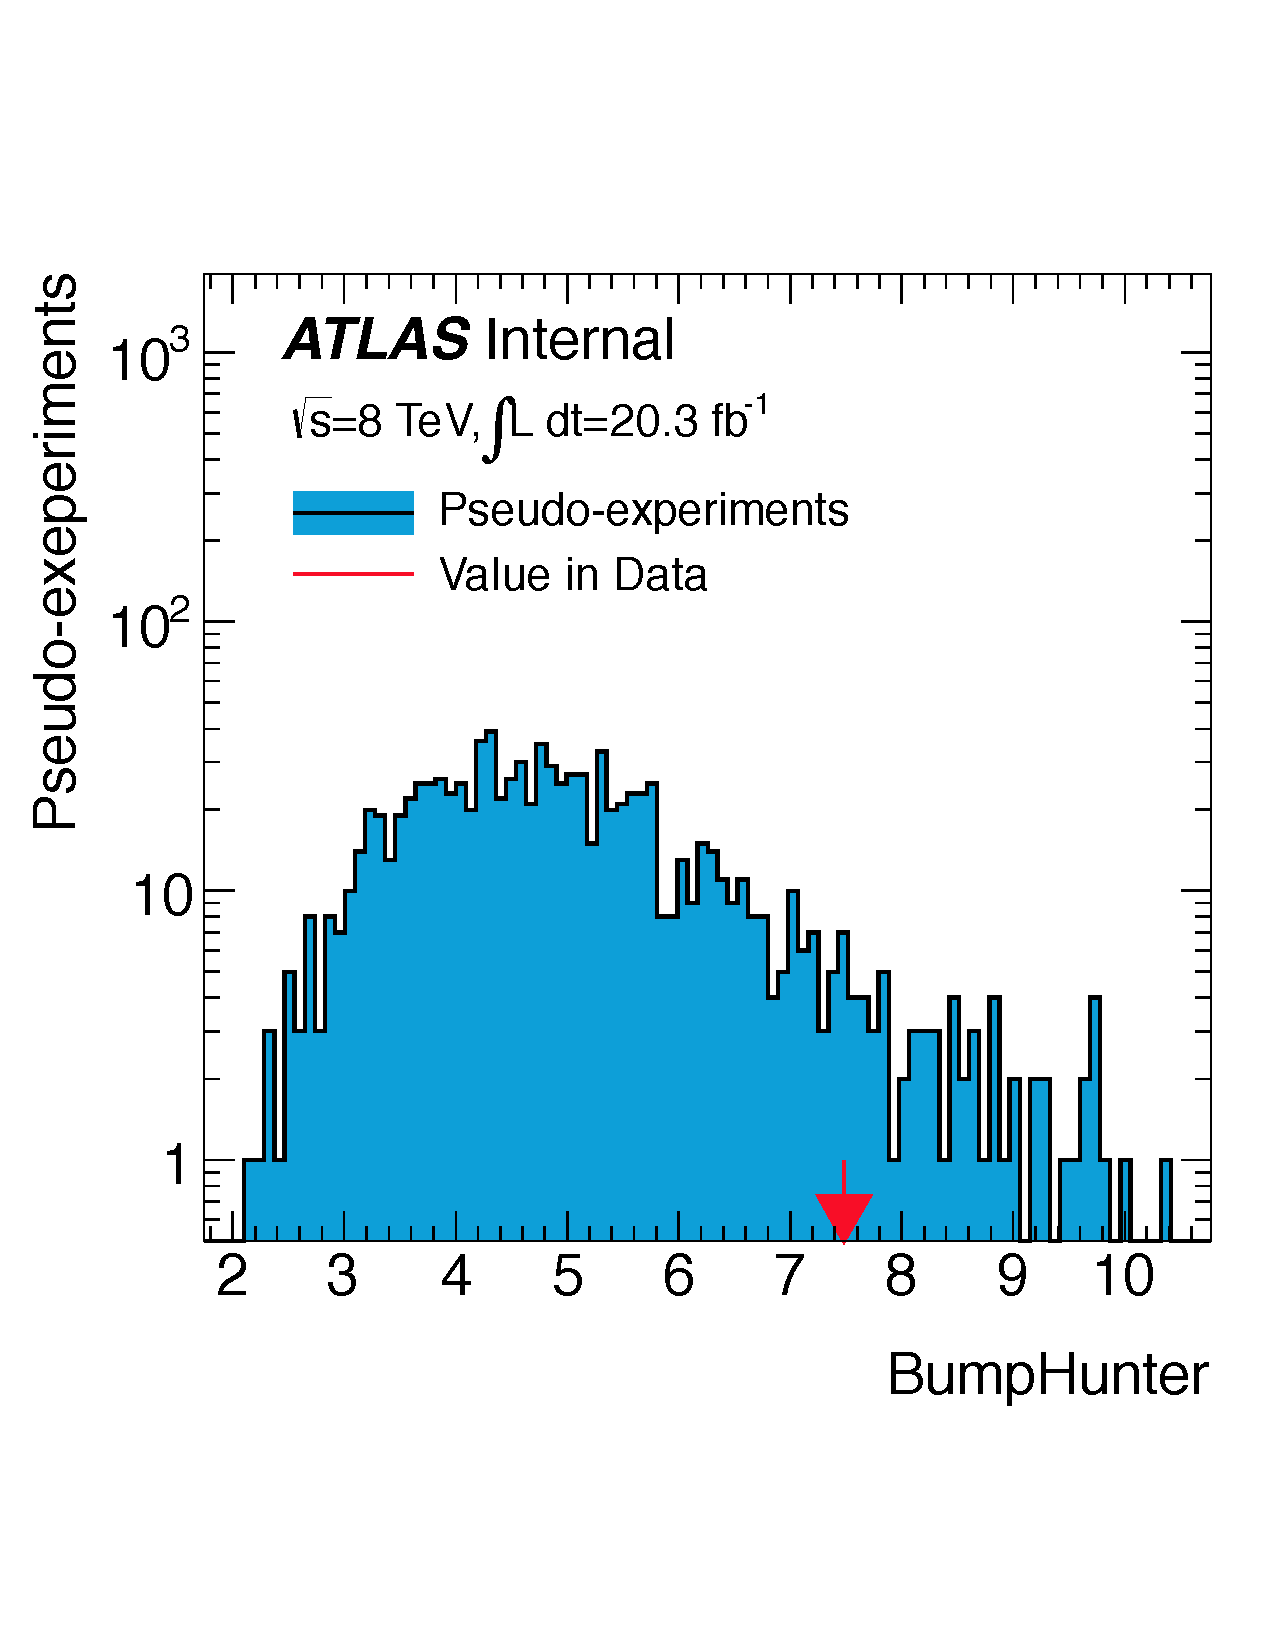
\includegraphics[width=0.75\textwidth]{figures/chapter_analysismethod/bumphunter}
%%        \caption{
%%            This diagram shows the bumphunter test statistics distribution, where the red arrow shows the observed value. 
%%        }
%%        \label{fig:teststats}
%%    \end{center}
%%\end{figure}
%%\FloatBarrier
%   
%   %The background fit, or parametrically, the SWiFT window size/Gaussian process lengthscale, is said to have passed the test if the largest signal the search is not sensitive to is within 3 $\sigma$ of the background error bands. 
%
%   %The smallest lengthscale value/SWiFT window size where the largest signal the search is not sensitive to stays in the error bands is the minimal SWiFT window/Gaussian Process fit value that can be used during unblinding. 
%
%\begin{figure}[!htb]
%    \begin{center}
%        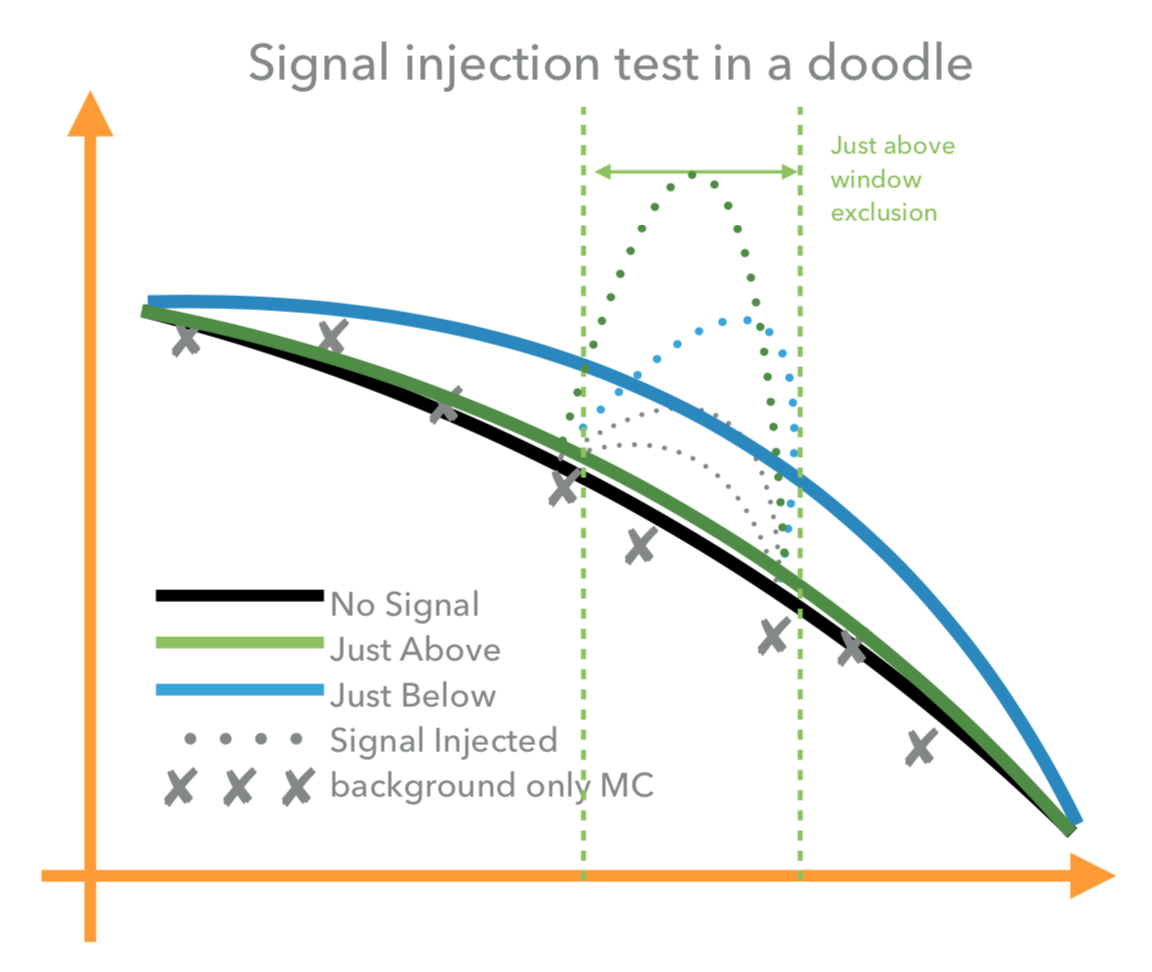
\includegraphics[width=0.7\textwidth]{figures/chapter_analysismethod/SignalInjectionTest}
%        \caption{
%            This figure shows a doodle of the procedure of the signal injection test. An increasingly large signal is injected to the background MC spectrum until the window exclusion procedure of bumphunter is triggered.
%        }
%        \label{signalinjection}
%    \end{center}
%\end{figure}
%\FloatBarrier
%
%\subsubsection{Spurious Signal Test} 
%    \label{sec:spurious}
%    %\epigraph{\textit{-``Test for signal extracted from the background estimation alone"}}
%
%    To measure the amount of possible false signal in the background modeling method, the spurious signal test is performed. The spurious signal test models the amount of signal that the background plus signal fit when no signal is present.  It statistically quantifies the stability of the background estimation. It is also sometimes used as a measure of the background fit error.
%
%Using the different variations of background only MC spectrum, a signal plus background fit is performed, the signal extracted is compared against the background error defined in the last section. The spurious signal test is considered passed if the signal extracted versus the background error ratio is $<$ 0.5.
%
%    The spurious signal is defined as the following:
%    
%    \begin{equation}
%        S_{spur} = S_{fit} - S_{template}
%    \end{equation}
%
%    Here $S_{fit}$ comes from the signal fit component of the background + signal fit, $S_{template}$ changes with the kind of analysis being performed. It is set to be 0 for a search.     
%    %The median of the 10000 pseudo experiment fit is taken to be the spurious signal value. 
%    %In the figure below, a sample spurious signal fit is shown~\ref{spurioussignal}.
%    %In general, the spurious signal has to stay within 50\% of the background error bands, defined as the error bands generated from the fitting of 10000 background MC pseudo experiment from the Poisson distribution with the background fit only.
%    %If the background fit stays within the 50\% requirement, it passes the spurious signal test.
%
%\begin{figure}[!htb]
%    \begin{center}
%        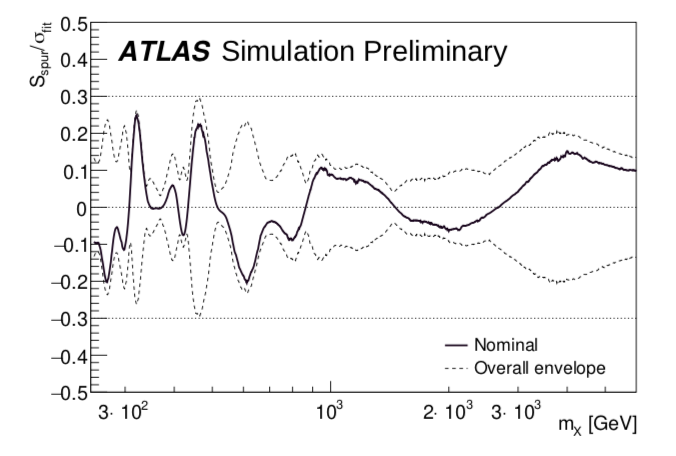
\includegraphics[width=0.75\textwidth]{figures/chapter_analysismethod/Spurious}
%        \caption{
%            This figure shows the example results of a spurious signal test. Here, the error $\sigma$ is defined as $\sigma_{tot} = \sqrt{\sigma^{2}_{fit}+ S_{spur}^{2}}$ ~\cite{ATL-PHYS-PUB-2020-028}.
%        }
%        \label{spurioussignal}
%    \end{center}
%\end{figure}
%\FloatBarrier
%
%After the data preparation steps and tests performed on background estimation. The mass spectrum and estimation are both ready for statistical testing for possible resonances. 
%
\section{Statistics Testing}
\label{section:stats}
Statistical testing is the quantification of the significance of any observed excess and the signal sensitivity exclusion presented in the data. The statistics testing of a hypothesis is related to the significance quantity Z:

\begin{equation}
 Z= \Phi^{-1}(1-p) 
 \label{eq:significance}
\end{equation}

Here, p is the probability of the background model to fluctuate and it describe the observation in relations to that. $\Phi$ is the conversion of the $p$-value into quantile of a cumulative Gaussian distribution. From here on, Z will be referred to as the significance and p will be referred to as the $p$-value.

There are two distinct statistics tests in a typical resonance search analysis. Each test is compared to a threshold value of Z. The two tests will be referred to as ``the search" and the ``limit setting". Details are described in the following sections.

%Before the Here, the null hypothesis is the hypothesis that include only known processes from the Standard Model hypothesis with no excess; the alternative hypotheis is the hypothesis that include both background and signal of a certain signal strength.

%\begin{itemize}
%    \item \textbf{1.  The Search}
%()corresponds to $p = 2.87 \cdot 10^{-7}$.


%the Bayesian tool is used for the dijetISR analyses, whereas the frequentist method is used for the dimuon analysis. 
%\end{itemize}

\subsection{The Search}
\label{sec:thesearch}
%\epigraph{\textit{-``The Rejection/Acceptance of the null hypothesis"}}

The search aims to look for model independent statistical excesses present in data. This test is implemented in comparison to the null hypothesis, where it is defined to be the Standard Model prediction. The search is implemented in a frequentist manner through the Bumphunter method~\cite{choudalakis2011hypothesis}. This section describes the statistics principle behind this test and details the bumphunting procedure. 

%From comparing the data test statistics value to pseudoexperiement, if the significance Z $>$ 5, the null hypothesis is rejected. Something beyond the Standard Model is observed in the data to a statistically significant degree, otherwise, the Standard Model prediction is accepted. In the Higgs boson analysis of 2012, a significance of Z $>$ 5 was observed in the search.


\subsubsection{The Search: The Statistics Principles}
The probability of having made a measurement in each bin can be described by a probability distribution. As each measurement is considered an independent event in a fixed data-taking period and physical variable value. The probability distribution takes the Poissonian probability distribution form:

\begin{equation}
 P(x=k|\lambda) = \frac{\lambda^{k}e^{-\lambda}}{k!} 
 \label{eq:Poissonian}
\end{equation}

Here, $\lambda$ is the expected value of the measured quantity $k$, $x$ is the quality being measured, e is Euler's number.

The test is implemented in a frequentist manner. It compares the observation outcome x with a fixed $\alpha$ of a probability distribution generated from pseudo-experiment. Psuedoexperiemnt are sample distributions drawn from the the Poissonian probability distribution of each bin. Test statistics can be calculated for each of these distribution. The value used to reject or accept the null hypothesis is quantity that is compared in relation to $\alpha$ called the $p$-value. Statistically, it is known to be a false-discovery probability(See Eq.~\ref{eq:test}). If the observation compared with the pseudo-experiment distribution is smaller than the critical $p$-value, an excess could have been discovered. The rejection criteria can be shown in the following mathematical form:

\begin{equation}
    P(x \ni w|H_0)<= \alpha 
    \label{eq:test}
\end{equation}

Here, $H_0$ is the null hypothesis, and alpha is the critical value below which an excess will be quoted. The value is usually taken to be 0.01 for the bumphunter experiment. It corresponds to a probability of 1\%. $x$ is the observed value. $w$ is all possible outcomes. 

\subsubsection{The Search: Test Statistics}
\label{teststatistics}

The test statistic is a function of the observable $x$, that describes the agreement between data and the model.  The $p$-value in~\ref{eq:test} can be rewritten as:
    
\begin{equation}
    p = P(T>=t_{0}| H_{0})
\label{eq:pvaluetestStats}
\end{equation}

Here, $H_0$ is the null hypothesis, $t_0$ is the test statistic above a certain test value, and T is the observed test statistic.

Equation~\ref{eq:pvaluetestStats} evaluate the $p$-value of the observed value. T is a function of the observed $x$ in the window. It's the probability of the observed test statistics obtaining a value at least as extreme as $t_{0}$. A small $p$-value refects a poor agreeement between the observed T value and the hypotheis $H_{0}$.

Various test statistics are available to quantify the level of agreement between an observation and a hypothesis. If the test is concerned with overall agreement between data and the model, the $\chi^{2}$ test or the log-likelihood of the Poissonian distribution are fitting candidates.

The bumphunter test statistic instead to quantifies localized excess. The test statistic is defined in a window and calculated for the bins within. It is a more powerful test for the kind of deviation expected in resonance hunting.

In a window defined from bin number m to n, the observed data and prediction can be given as the following: 
    \begin{equation}
         d= \sum_{i=m}^{n} d_i 
    \end{equation}

    
    \begin{equation}
         b= \sum_{i=m}^{n} b_i
    \end{equation}

    Here d is the total number of events in the window observed, where $d_i$ is the count in each of the bins from m to n. 
    Here b is the total number of events in the window predicted, where $b_i$ is the event count in each of the bins from m to n.
    
    Assuming the observed counts in each bin follow a Poissonian distribution, the test statistic is:

\begin{equation}
    t^{\textrm{BH}}=
    \begin{cases} \sum_{n=0}^{d} \frac{b^{n}}{n!} e^{-b} &  \textrm{for $d < b$}
    \\
    \sum_{n=d}^{\infty} \frac{b^n}{n!} e^{-b} &  \textrm{for $b \leq d$}
    \end{cases}
\end{equation}

    The above expression can be represented by the Gamma function($\gamma$): 

\begin{equation}
    t^{\textrm{BH}}=
    \begin{cases} 1-\gamma(d+1, b) &  \textrm{for $d < b$}
    \\
    \gamma(d,b) &  \textrm{for $b \leq d$}.
    \end{cases}
\end{equation}
    

    The $p$-value of the bumphunter test statistic is evaluated for every windows from two-bin wide to half the spectrum($t^{\textrm{BH}}$). The overall bumphunter test statistic is defined by the to be the log of the smallest $p$-value calculated from the smallest $p$-value window, and can be represented as the following($t^{\textrm{BH}}_{min}$):

    \begin{equation}
        t_{min}^{\textrm{BH}} = - \ln(t_^{\textrm{BH}}_{\textrm{min}}) 
    \end{equation}

    Significance Z and the $p$-value can be calculated from this test statistic in Eq.~\ref{eq:pvaluetestStats} and thereby provide the probability that the SM hypothesis could have generated data this unlikely or more. %the null hypothesis is rejected, otherwise, it is accepted.

    %In addition to the bumphunter test statistics, there is the tailhunter, KS, Jeffreys and no sidebands bumphunter that can also be chosen for different signals searched for in other physics analyses. More information can be found in the Bumphunter paper\cite{choudalakis2011hypothesis}.

    \subsubsection{The Search: The Bumphunting Procedure}
    % Look up the bumphunter fit. 
    The bumphunting procedure is defined to look for excesses as defined by the bumphunter statistics~\cite{Pachal:2063032}.

    1.  First a background model fit is performed. (See Section~\ref{sec:backgroundest}). The $\chi^{2}$ of the fit is verified to have a $p$-value $>$ 0.01. Otherwise, the fit will be revised or moved to an alternative method.

    2.  If the background fit passes the $\chi^{2}$ test, the bumphunting test can begin. In all defined windows, bumphunter test statistic and their $p$-values are calculated. If the overall bumphunter test statistic has a $p$-value above 0.01, the procedure stops, no excess is found. Alternatively, if any one of the windows has  $p< 0.01$, the window most discrepant window (the window with the lowest $p$-value) is removed, and the fit is reperformed. If the new fit with the window removed has a $p$-value above 0.01, it shows the discrepancy is completely contained in the window removed.

    3. After reperforming the fit with the window removed, if an overall bumphunter statistics $p$-value is found to be over 0.01, Stop. A local discrepancy may have been discovered in the removed window. Otherwise, if the newly discovered most discrepant window is adjacent to the window removed, it demonstrates that the signal peak may still be outside of the window, one more bin of window exclusion will be added to the removed window. If the newly discovered most discrepant window is not adjacent to the window removed, one bin of each side is added to the original removed window. The fit is re-performed with the new window removed. This step is repeated until either the $p$-value of the fit with the removed window has a $p$-value above 0.01, or no additional window could be added to the exclusion because all bins has been added to the removal window.

    Summarizing from the above, three end results are possible in the search test:

    1. If no window is excluded and the fit has a bumphunter $p$-value statistics above 0.01. No excess is found. 

    2. If there is one excluded window and a background fit with a bumphunter statistics $p$-value of above 0.01. An excess up to a certain significane is quoted.

    3. In all other scenarios, more tests are required. The background model fit could be problematic and need further testing.  

\section{Limit Setting}
\label{sec:limits}

%\epigraph{\textit{Finding signal strength value where the alternative hypothesis is rejected to a 95\% confidence level}}


%The signal strength can also be represented as a cross-section or cross-section in fiducial volume for reinterpretation for different models. 
%The limit setting results consist of a 95\% confidence upper limit bound on signal strength over the resonance masses and an expected limit of median significance along with statistical uncertainties with the null hypothesis. 
%It is possible to compare the observed 95\% upper limit against the expected limit. The comparison between the bands and the upper limit line can be seen as a discovery test, as if no beyond the Standard Model excess is seen, the upper limit line would stay between the 5 $\sigma$s error band in the expected limit. 

The limit setting can be performed in two different ways, the Bayesian statistical way and the frequentist way. While the interpretation and implication of the results made with the different methods are different, the results produced are designed to be comparable across different analyses. 

The Bayesian method is used for the dijetISR analysis(Chapter~\ref{chapter:dijetISR}) and the frequentist method is used for the dimuon analysis(Chapter~\ref{chapter:dimuon}). A description of the dimuon frequentist limit is given as below. 
%The 95\% confidence level corresponds to a critical $p$-value of 0.05 or a Z value of 1.64.

%The limit is a hypothesis testing procedure that test both the compares the null hypothesis of absence of signal ($H_{0}$) to the hypothesis where there is a signal($H_{1}$). 
%The limit is a projection of the $H_0$ and $H_1$ hypothesis in either the cross-section or the signal strength axis. This provide another way to discuss signal discovery, and information on an 95\% confidence limit in the If $H_1$ shows agreement with $H_{0}$ when fluctuation is taken into account, the 
%Even in the absence of a signal, a statement can be made about the signal strength value that is ruled out by the signal+background. 
%
%The limit setting procedure can be done in both the frequentist and Bayesian way on ATLAS, and in the analyses presented, the dimuon analysis is done in the frequentist way, whereas the dijet analysis is done in the Bayesian way. 

%\subsection{Bayesian limits}


\subsection{Frequentist Limits}
\label{sec:freq}
%The coverage probability is the fraction of interval in an ensemble such that the true parameter is contained. Confidence intervals are constructed to have a coverage probability greater than or equal to the given confidence level. 
%The limit is a statement on where the observed data lies given all the other possible outcomes given a hypothesis. The frequentist limit state that given an ensemble of identical experiments, the true value of the signal strength should be under the observed limit 95\% of the time. 
%The 95\% CL upper limit is result of a procedure which if run in hypothetical similar experiments would include (exclude) the true value 95\% (5\%) of the time.

%The confidence interval of a frequentist limit is obtained by a finding a coverage probability that include the true value 95\% of the time. The unit chosen for this procedure is signal strength over the signal mass points. 

The following subsection describes the test statistics used for the limit setting. A formulation of the traditional frequentist calculation is presented. The Asimov approximation method used to approximate the frequentist limit from a representative dataset is described, which is the ATLAS standard, and it saves computing resources. The formulae for the limit calculation using this method are given. Adaptation with the Gaussian Process is also discussed. 

\subsubsection{Frequentist Limits: The Test Statistics}
\label{sec:freqTestStats}

The probability distribution of the observable $x$ in each bin of the histogram can be given by a Poissonian probability distribution. This probability distribution is a function of many parameters, including the signal strength, and other systematic uncertainty parameters, for example, the variation in luminsoity. As these variable are not the target parameter where limit is set, they are known as the nuissance paramters. From the Poissonian distribution, its likelihood function can be parameterized as such, with the predicted signal event and background events made explicit:

\begin{equation}
    L(\mu, \theta) =  \prod_{i=0}^{N} \frac{(\mu \cdot s_{j} + b_{j})^{n_j}}{n_{j}!}e^{(-\mu \cdot s_j + b_j)} \prod_{k=1}^{M}\frac{u_{k}}
{m_{k}!} e^{(-u_{k})}
\label{eq:likelihood}
\end{equation}

Here, $L$ is the likelihood product from the target distribution multiplied by systematic parameter distributions, $\mu$ is the signal strength, $s_j$ is the number of expected signal events in the jth bin, $b_j$ is the number of expected background events in the jth  bin, $n_j$ is the number of observed events in each bin; N is the total number of bins. The likelihood is also affected by variations in other parameters, which include sysmstatic uncertainty terms such as imprecise luminosity measurement or energy correction uncertainties. These are not the targeted signal strength and are often known as the nuissance parameters. here, $u_k$ is the predicted value by the model, and $m_{k}$ is the observed value. 

%The likelihood is also affected terms in other distributions, these
%are not the target distribution and can be accounted for as the nuisance parameters, which includes luminosity uncertainties etc. 

The most probable value of the parameters are those that maximize the likelihood function. However, since in limit setting, the only parameter we are interested in learning about is the signal strength, the influence from the unknown true value of the nuisance parameters can be taken into account or eliminated. As optimizing the true likelihood is often computationally expensive, a ``profiled likelihood" function is constructed. This quantity, when maximized, gives the same effect as maximizing the true likelihood. 

\begin{equation}
\lambda(\mu) = \frac{L(\mu, \hat{\hat{\theta}})}{L(\hat{\mu}, \hat{\theta})}
\label{eq:profilelikelihood}
\end{equation}

Here, $\hat{\hat{\mu}}$ is the $\theta$ that maximizes L for $\mu$ specified. the denominator is the maximized unconditional likelihood function, where $\hat{\mu}$ and $\hat{\theta}$ are the parameter values that would maximize the unconditional likelihood function regardless of specific $\mu$ values.

%To aid the optimization process and also to reflect the nature of the excess search experiment that neglects negative signal event value, the test statistics defined as the following, the negative log taken on the likelihood ratio aid the optimization computing procedure.
To aid the optimization process, it is usually the negative log of the profiled likelihood that is used for the limits calculation:

\begin{equation}
    q_{\mu} = -2 \ln \frac{L(\mu, \hat{\hat{\theta}})}{L(\hat{\mu}, \hat{\theta})}
\label{teststats}
\end{equation}


\subsubsection{The Frequentist Limits: The Limits Formulae}
\label{sec:freqlimits}

%From this test statistics, certain assumed signal strength $\mu$ in the nominator returns a 95\% confidence in the rejection, this is calculated for different signal mass points and is called the observed limit. The signal strength of median significance along with the fluctuation is called the expected limit. 
The formulae for the limits calculation is given below:

\begin{itemize}


\item \textbf{The Observed 95\% Upper Limit}
\begin{equation}
\mu_{up/lo} = \hat{\mu} +- \sigma\Phi^{-1}(1-\alpha/2)
\end{equation}

here, $\mu$ is the signal strength, up/lo is the upper or the lower 5\% confidence limit. 

\item \textbf{The Expected Median Limit}
\begin{equation}
    \mathrm{med}[\mu_{up}|\mu'] = \mu' + \sigma\Phi^{-1}(1-\alpha) 
\end{equation}
here, $\mu'$ is the expected signal strength.


here, $\mathrm{med}$ is the  median of the observed limits.

\item \textbf{The Expected Limits Significance}
\begin{equation}
    \mathrm{band}_{N\sigma} = \mu' + \sigma(\Phi(1-\alpha)+-N)
\end{equation}

\end{itemize}


Here, $\mu$ is the signal strength being considered, $\alpha$ is the significance associated with 95$\%$ confidence and the median significance respectively, $\Phi$ is the cumulative Gaussian distribution where the observed $p$-value lies.

Note that the calculation of the denominator in~\ref{eq:likelihood} is CPU-intensive, and can be approximated.


\subsubsection{The Frequentist Limits: The Asymptotic distribution}
\label{sec:asymp}


From the Wald theorem, the test statistic can be approximated: 

\begin{equation}
-2\ln(\lambda(\mu))= \frac{(\mu- \hat{\mu})^{2}}{\sigma^{2}} +O(1/\sqrt{N})
\label{eq:wald}
\end{equation}

Here, $\mu$ is the observed value, whereas the $\hat{\mu}$ is the expected strength that would maximize the likelihood, $\sigma$ is the expected spread in the distribution. 

If the terms in O are neglected, the test statistic will then asymtotically follow a non-central chi-square distribution, derivation is in~\cite{2011}: 

\begin{equation}
    f(q_{\mu}) = \frac{1}{2\sqrt{q_{\mu}}} \frac{1}{\sqrt{2\pi}} [exp(-\frac{1}{2}(\sqrt{q_{\mu}}+ \sqrt{\Lambda})+ exp(-\frac{1}{2}(\sqrt{q_{\mu}-\sqrt{\Lambda}})^{2})]
\end{equation}
Here, $\Lambda$ is the non-centrality term, it can be shown that it can be estimated to be:

\begin{equation}
    \Lambda=2\ln(\lambda_{A}(\mu))
    \label{eq:Lambda}
\end{equation}

Where $\lambda_{A}$ is the likelihood calculated from the asymtotic distribution. A detailed proof can be found in~\cite{2011}. 

%\[ \lambda_{A}(\mu) = \frac{L_{A}(\mu, \hat{\hat{\theta}})}{L_{A}(\hat{\mu}, \hat{\theta})} \]


%Following certain estimation, the non-centrality term, \Lambda, can be given by the following:


%Following from this, it can be shown mathmatically the median significance, the error bands, as well as the upper limit exclusion can be given as the following: 


%The upper limit is given by: 
%\[ \

%The median significance of the expected limit is given by
%\[ \Lambda = \frac{(\mu- \hat{\mu})^{2}}{\sigma^2}=-2ln{lambda} \], where mu is the expected value, this is known as the asimov dataset. 


%\begin{figure}[!htb]
%    \begin{center}
%        \includegraphics[width=0.75\textwidth]{figures/chapter_analysismethod/asimovApproximation}
%        \caption{
%			Generation showing convergence of the Asimov dataset and the median significance dataset from full generation. .
%        }
%        \label{fig:Model_figure}
%    \end{center}
%\end{figure}
%
%
%\[ Z^{2}_{median} = -2ln{\lambda_{median}} \]
%
%As can be shown from the MC generation plot here, the median conversed 
%
%Using the above approximation, one distribution can be used instead of a large amout of ensemble data, the above is known as the Asimov dataset. 


%There are some special cases where the 

%From the Wilk's theorem, the upper limit on the signal strength $\mu_{95}$ can be given as the following:


\subsubsection{Frequentist Limit: The Asimov dataset}
\label{sec:asimov}

The finding of $\hat{\mu}$ in the denominator in ~\ref{teststats} is CPU intensive. The dataset is large with many dimensions. The Asimov dataset reduces the calculation here by showing that $\hat{\mu}$ can be approximated by $\mu'$, the expected value of the strength parameter. From this, CPU intensive calculation of the $p$-value can be avoided. Significance and thus the upper limit and the observed limit fluctuation can be reduced to simple formulae that only
require calculations from the representative Asimov dataset. 
A proof is given in the following section, and the formulae used for the upper limit and expected limit calculation in this thesis are included in the end. 

%From the definition, true parameters values will result in the maximum likelihood and therefore the derivative of the ${L}$ will be equal to 0. 
%
%\begin{equation}
%\frac{\partial{L}}{\partial{\theta_{j}}} \sum_{i=0}^{N}(\frac{n_{i}}{\nu_{i}}-1) \frac{\partial{\nu_{i}}}{\partial{\theta_{j}}}+ \sum_{i=0}^{N}(\frac{m_{i}}{u_{i}}-1) \frac{\partial{u_{i}}}{\partial{\theta_{j}}} =  0 
%\end{equation}
%
%Here, $n_i$ is the number of events in the bin i in the signal region, and N is the total number of bins, and m is the number of events in bins in the control region may help further constrain the background, M is the maximum number of bins. $\nu$ is the expected event number and $u_{i}$ is the expected number of events in bin i. 
%
%The maximal likelihood value for $n_{i,A}$ and $m_{i,A}$ in the Asimov distribution is associated with their expectation value. 
%
%\begin{equation}
%    n_{i,A} = E[n_{i}] = \nu_{i} = \mu s_{i}(\theta) + b_{i}(\theta)
%\end{equation}
%
%\begin{equation}
%    m_{i,A} = E[m,i] = u_{i}(\theta)
%\end{equation}
%
%The optimal parameters $\theta$ can be estimated through large-size Monte Carlo generation. And it is called the Asimov dataset.
%The only missing part from the above estimation is $\sigma$, which can be approximated as the following: 
%Since, 
%
%\begin{equation}
%    \lambda_{A}(\mu) = \frac{L_{A}(\mu, \hat{\hat{\theta}})}{L_{A}(\hat{\mu}, \hat{\theta})}
%= \frac{L_{A}{\mu, \hat{\hat{\theta}}}}{L_{A}(\mu', \theta)}
%\end{equation}
%
%
%From Eq.~\ref{eq:wald} and Eq.~\ref{eq:Lambda}:
%\begin{equation}
%2\ln(\lambda_{A}(\mu)) \approx \frac{(\mu-\mu')^{2}}{\sigma^{2}}=\Lambda
%\end{equation}
%
%$\sigma_{A}$ can therefore be approximated:
%
%\begin{equation}
%    \sigma_{A}^{2} = \frac{(\mu-\mu')^{2}}{q_{\mu,A}}
%\end{equation}
%
%When there is no signal, $\mu'$ is taken to be zero. 

%Following from the above, the test statistic, the upper limits, the discovery median significance can all be found through substituting $\hat{\mu}$ as $\mu'$ by the Asimov method. Below are additional results derived from the above, but quoted without derivation.


%As these result derives directly from the above, only the results are quoted here. 
Below are the results quoted from~\cite{2011}, a detailed derivation can be found there. 

\begin{itemize}
    \item \textbf{The Test Statistics Distribution}

\begin{equation}
    F(t_{\mu}| \mu) = 2\Phi(\sqrt{t_{\mu}})-1
\label{eq:teststatistics}
\end{equation}

Here F is the distribution of the statistics, $t_\mu$ is the test statistic at the given $\mu$ value of the distribution. 

\item \textbf{The P-value of a Hypothesized $\mu$ for an Observed Value $t_\mu$}

\begin{equation}
p_{\mu} = 1-F(t_{\mu}| \mu)=2(1-\Phi(\sqrt(t_{\mu})))
\end{equation}


\item \textbf{The Significance}

\begin{equation}
Z_{\mu} = \Phi^{-1}(1-p_{\mu})  = \Phi^{-1}(2\Phi(\sqrt{t_{\mu}})-1)
\end{equation}

\end{itemize}

From this calculation, the limit calculation in the above Section~\ref{sec:limits} can be utilized for a limit calculation. 

%\subsection{The Search (discovery test)}
%A hypothesis is said to be rejected if its $p$-value is below a certain threshold z value of alpha. This is the basis of the discovery test.
%Using the test statsitics:
%
%
%
%\begin{equation}
%\[ Z_{0}= \Phi(1-p_{0})= \sqrt(q_{0}) \]
%\end{equation}



%In the experiment, statistical fluctuation need to be taken into account, it can either be taken as that the data has room to fluctuate, or that the expected value from the model can fluctuate and change. Either way, the sigificance will fluctuate even if $\mu'$ is assumed to be true and hold fixed. In the analysis, it's taken that data will be fluctuating. 
%
%In the case where there is assumed that there is no background. Using the fluctuation, the significance can be calculated as the following: 
%
%\begin{equation}
%Z_{0}= 
%\begin{cases}
%    1& \text{\mu* \sigma    \hat{\mu}\gt 0}
%    2& \text{0    \hat{\mu}<0}
%\end{cases}
%\end{equation}


%For the expected limit test, the significance can be written as:
%\begin{equation}
%    \[ Z_{0}(\mu'+N\sigma) = med[Z|\mu'] +N \] 
%\end{equation}
%

%\begin{equation}
%    \[ max[Z_{0}(\mu'+N\sigma) = med[Z|\mu'] -N, 0] \] 
%\end{equation}

\subsubsection{Frequentist Limits: Gaussian Process Adaptations}
    The Gaussian process has been  shown to be able to be incorporated within the Asimov method of frequentist limit setting~\cite{frate2017modeling}.
    In Figure~\ref{fig:chi2}, the likelihood ratio in the Gaussian process~\ref{eq:gplikelihood} is a proxy for the profile likelihood ratio used in the Asimov limit. The likelihood came from the ~\ref{eq:loglikelihood} in the Gaussian Process section above.  It can be seen that it approximately follows the $\chi^{2}$ distribution, satisfying a requirement that follows from the Wald approximation that allows for the Asimov approximation of limits.

    \begin{figure}[!htb]
        \begin{center}
            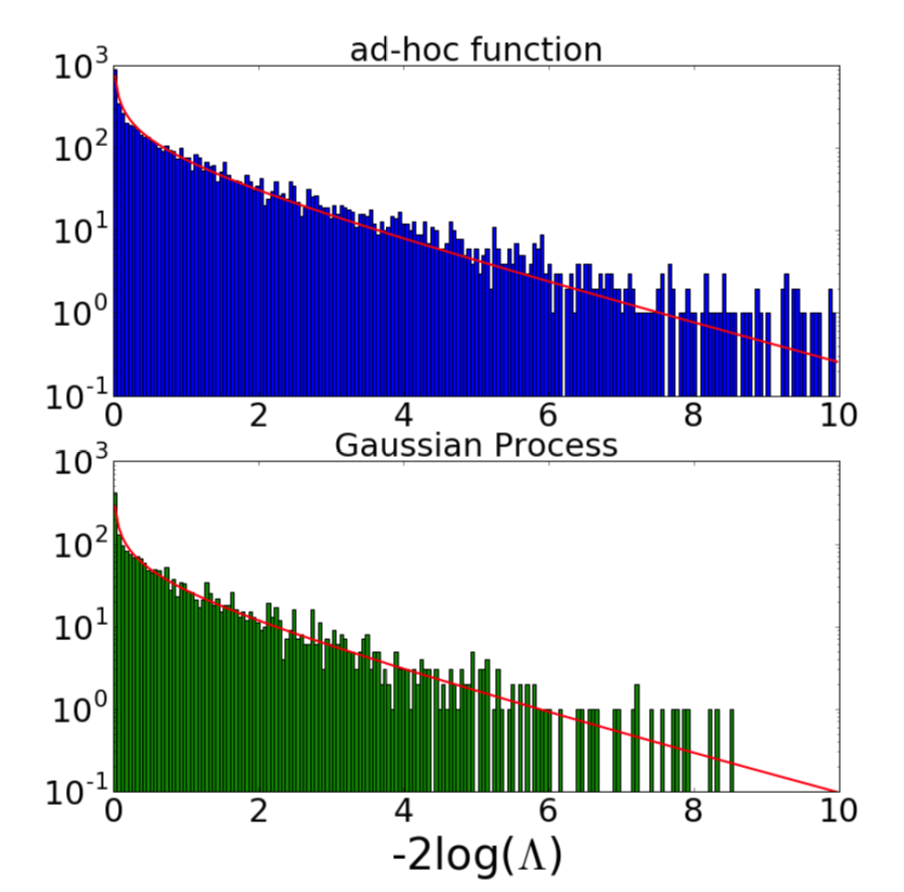
\includegraphics[width=0.75\textwidth]{figures/chapter_analysismethod/chi2}
                \caption{
                This figure shows the negative log of the $\Lambda$ which is an approximation of the measure of the profiled likelihood ratio defined in~\ref{eq:profilelikelihood}. The top part is the distribution for background only pseudo-experiments, whereas the bottom is the background and signal distribution. They show a reasonable agreement to the $\chi^{2}$ fit, a required condition for the Asimov approximation for a frequentist limit setting~\cite{frate2017modeling}. 
            }
            \label{fig:chi2}
        \end{center}
    \end{figure}
    \FloatBarrier

    A new test statistic for Gaussian Process that is parametrized by the kernel hyperparameters is used instead for limit setting:

\begin{equation}
    -ln(\Lambda) \textrm{, where }\Lambda= \frac{L_{\textrm{GP signal + bkg fit}}(\mu, \hat{\hat{\theta}})}{L_{\textrm{GP bkg fit}}(\hat{\mu}, \hat{\theta})})
\label{eq:gplikelihood}
\end{equation}

Here, $\ln(\Lambda)$ is the new test statisitics used for the limit setting L is the likelihood defined in Eq.~\ref{eq:loglikelihood}. The numerator is the likelihood with both the background and signal kernel, whereas the denominator is likelihood with just the background kernel. 

With the above procedure in place, actual data from analysis is ready to be analyzed for resonance in the dijetISR and dimuon channels.

